\section{Case Study: Inertia-Wheel Pendulum}
\label{sec:iwp}

In this section, we validate the proposed control design framework on the
problem of swinging-up and stabilizing the inverted position of an inertia wheel
pendulum (IWP), shown in Fig.~\ref{fig:iwp}. We provide experimental results
from simulation and real-world hardware in order to thoroughly demonstrate the
efficacy and robustness claims of Bayesian inference. 
%
We use the deterministic solution for \textsc{NeuralPbc} as the baseline
on which we compare the performance of the Bayesian solution.


\subsection{System Model}
\label{ssec:model}

The IWP mechanism consists of a pendulum with an actuated wheel instead of a static
mass.
%
The wheel has mass $m$, which is connected to a massless rod of length \(l\). 
%
The position of the rod is denoted by the angle \(q_1\) measured with
respect to the downward vertical position.
%
The position of the wheel \(q_2\) is measured with respect to the vertical
line through the center of the wheel.

The Hamiltonian of the IWP is given by Equation ~\eqref{eq:system_hamiltonian}
with $n=2$ and
%
\begin{equation*}
    M = \bmat{I_1 & 0 \\ 0 & I_2},
    \;
    G = \bmat{-1 \\ \phantom{-}1},
    \;
    V(q) = mgl \left( \cos q_1 - 1 \right),
\end{equation*}
%
and $p = \left(I_1 \dot{q}_1,I_2 \dot{q}_2\right)$. 
%
We denote the state of the system as $x = (q_1, q_2, \dot{q}_1, \dot{q}_2)$.
%
The parameters \(I_1\) and \(I_2\) denote the moment of inertia of the pendulum
and the wheel, respectively, and \(g\) is the gravitational constant.
%
% The wheel has mass $m$, which is connected to a massless rod of length \(l\). 
%
The equations of motion of the IWP can be written as 
%
\begin{equation}
    % \begin{aligned}
    %     I_1\ddot{\theta}_1 &= -mgl \sin(\theta_1) - u, \\
    %     I_2\ddot{\theta}_2 &= u
    % \end{aligned}
    % \bmat{I_1 & 0 \\ 0 & I_2} \bmat{q_1 \\ q_2} + \bmat{-mgl \sin q_1 \\ 0} = \bmat{-1 \\ \phantom{-}1} u, 
    M \bmat{\ddot{q}_1 \\ \ddot{q}_2} + \bmat{-mgl \sin q_1 \\ 0} = Gu, 
    \label{eq:iwp_dynamics}
\end{equation}
%
where the control input \(u\) is the torque applied to the inertia wheel.
%
The desired equilibrium $x^\star = (q^\star, 0)$ is the origin, which
corresponds to the upward position.
%
The nominal system parameters are estimated to be $I_1 = 0.0455$ kg-m$^2$, $I_2
= 0.00425$ kg-m$^2$, and $mgl = 1.795$ N-m. 
%
% The control objective is to ensure that closed-loop trajectories
% of~\eqref{eq:iwp_dynamics} passes through a neighborhood of $x^\star$,
% at which point a linear stabilizing controller can be employed to asymptotically
% stabilize the system at $x^\star$.
%

\begin{figure}[t]
    \centering
    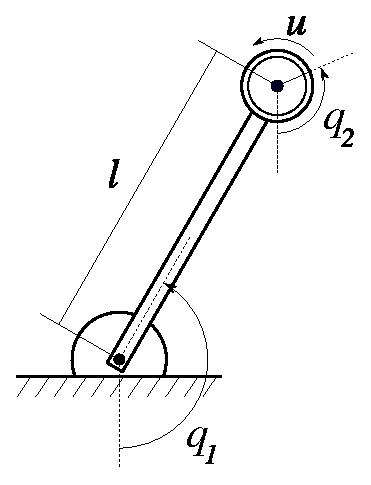
\includegraphics[width=0.25\linewidth]{figures/iwp.eps}
    \caption{Schematic of the inertia wheel pendulum. Only the joint $q_2$ is actuated, and $q_1$ is not.}
    \label{fig:iwp}
\end{figure}

% The joint $q_2$ in our hardware implementation is actuated by a Nanotec DFA90
% brushless DC motor through a belt drive system.
% %
% The motor is mounted concentrically with the joint $q_1$ to minimize $mgl$. 
% %
% The actuator torque (current) is controlled by Maxon EPOS2 70/10. 
% %
% The nominal system parameters are estimated to be $I_1 = 0.0455$ kg-m$^2$, $I_2
% = 0.00425$ kg-m$^2$, and $mgl = 1.795$ N-m. 


\subsection{Case Study}

We begin by demonstrating the \textsc{NeuralPbc} framework outlined in
Section~\ref{ssec:ml-pbc} on the IWP system. 
%
In this setting, the surrogate $H_d^\theta$ for the closed-loop energy function
is determined by solving the optimization
problem~\eqref{eq:neural_pbc_finite_optim}, and the corresponding control law is
applied on the system given by~\eqref{eq:iwp_dynamics}.
%
We apply this control law in conjunction with the Linear Quadratic Regulator
(LQR), the latter of which is activated when the trajectories enter a
neighborhood of $x^\star$.
%
Two case studies are performed: 1) solving~\eqref{eq:neural_pbc_finite_optim}
through stochastic gradient descent (deterministic training from
Section~\ref{sssec:ml-pbc-deterministic}), and 2)
solving~\eqref{eq:neural_pbc_finite_optim} through Bayesian learning
(Section~\ref{sssec:ml-pbc-bayes}).
%
The results from both case studies are compared to showcase the effectiveness of
\textsc{NeuralPbc} and the robustness benefits of Bayesian learning.


\subsubsection{Training Setup}

The energy-like function $H_d^\theta$ is a fully-connected neural network with
two hidden layers, each with the \textsc{Elu} activation function. 
%
% There are, in total, 137 parameters to learn. 
% %
% They are initialized according to the Glorot
% (Xavier)~\cite{glorot2010understanding} scheme.
%
% The objective of the optimization problem~\eqref{eq:neural_pbc_finite_optim}
% consists of $\ell_{\textrm{set}}$ given by Equation~\eqref{eq:set_distance},
% with the set $\mathcal{S}$ chosen as a ball of radius $r = 0.01$ around
% $x^\star$ in the standard norm topology.
%
A uniform distribution in $[-2\pi, 2\pi] \times [-2\pi, 2\pi] \times [-10, 10]
\times [-10, 10]$ is chosen as the probability distribution from which samples
of initial states $x_0$ are drawn for the \textsc{DAgger} strategy.
%
In each gradient descent step, a batch of 4 initial states $\{x_0\}$,
generated by the state sampling technique in~\ref{sssec:ml-pbc-sampling}, are
integrated forward with a time horizon of $t \in [0,3]$ seconds. 
%
In the Bayesian framework, the standard deviations $\sigma_{\zeta}$ of system
parameters $\zeta = [I_1, I_2, mgl]$ are chosen to be $10\%$ of the nominal system
parameters given in Section~\ref{ssec:model}.
%
Moreover, we train on trajectories per the SDE in~\eqref{eq:sde_initial} with
measurement error represented by Wiener process with standard deviation of 0.001
and 0.02 on the joint angles and velocities, respectively.
%
% In each gradient descent step, a batch of 4 initial conditions $\{x_0\}$
% generated by \textsc{DAgger} is integrated forward with using the Tsitouras
% $5(4)$ Runge-Kutta solver with a time horizon of $t \in [0,3]$ seconds. 
%
% The cost function is then computed and back-propagated using the
% AD-assisted adjoint method implemented in
% \verb|DiffEqFlux.jl|~\cite{DBLP:journals/corr/abs-2001-04385}.
% %
% In the Bayesian learning framework, we draw samples from the posterior and
% back-propagate through the gradients of the \textsc{Elbo} using the
% \textsc{ADVI}~\cite{kucukelbir2015automatic} scheme provided in
% \verb|Turing.jl|~\cite{turing}. 
%
The trainings are terminated when the loss function $\ell$ and the \textsc{Elbo}
converge for the deterministic and Bayesian trainings, respectively.
%
The hyperparameters for the deterministic and Bayesian \textsc{NeuralPbc}
trainings are shown in Table~\ref{tab:training_setup_neuralpbc}.
%
It can be seen that the Bayesian training effectively learns with smaller neural
network size and fewer data than the deterministic training.
\begin{table}[tb]
    \centering
    \caption{\textsc{NeuralPbc} training setup for deterministic and Bayesian frameworks}
    % \rowcolors{2}{}{Wheat1}
    \begin{tabular}{lcc}
      \toprule
    %   & \multicolumn{2}{c}{Framework} \\
    %   \cmidrule(lr){2-3}
       & Deterministic & Bayesian \\
      \midrule
        $H_d$ neural net size & (6, 12, 3, 1) & (6, 5, 3, 1)\\
        Learned parameters & 133 & 128  \\
        Optimizer & \textsc{ADAM} & DecayedAdaGrad\\
        Initial learning rate & 0.001 & 0.01\\
        Replay buffer size & 400 & 50\\
      \bottomrule
    \end{tabular}
    \label{tab:training_setup_neuralpbc}
  \end{table}

\subsubsection{Simulated Experiments}

%
The performance of the controllers obtained from the deterministic and Bayesian
trainings are compared as follows.
%
% Both frameworks are trained with the nominal system parameters given in
% Section~\ref{ssec:model}.
%
We evaluate the performance of both trainings with parameter uncertainties
on $I_1, I_2$ and $mgl$. 
%
We introduce these uncertainties by moving the average
system parameters by $\pm 10\%$ to $\pm 50\%$ with increments of $10\%$. 
%
For each average system parameter, we sample uniformly with a $\pm 5\%$ support
around the average system parameters. 
%
This helps test the performance of the controller with various combinations of
$I_1, I_2$ and $mgl$.
%
On top of the system parameter uncertainties, we introduce measurement noise
represented by a Wiener process with standard deviation of $0.001$ and $0.02$ on
the joint angles and velocities, respectively. 
%
Fig.~\ref{fig:comparison_neuralpbc} shows the performance of deterministic and
Bayesian trainings using an accumulated quadratic loss of the form
\begin{equation} J_T = \frac{1}{2}\int_0^T \left(x^\top Qx + u^\top Ru \right) dt.
  \label{eq:performance_metric} \end{equation}
%
The controller derived from the Bayesian training is marginalized over 10
parameters sampled from the posterior distribution. 
%
As shown in Fig.~\ref{fig:comparison_neuralpbc}, the Bayesian training
effectively incurs less cost for large error in system parameters.
%
Moreover, the error band on the cost of the Bayesian training is smaller than
that of the deterministic training, demonstrating that the marginalized
controller is more robust against measurement noise.
%   
\begin{figure}[tb]
    \centering
    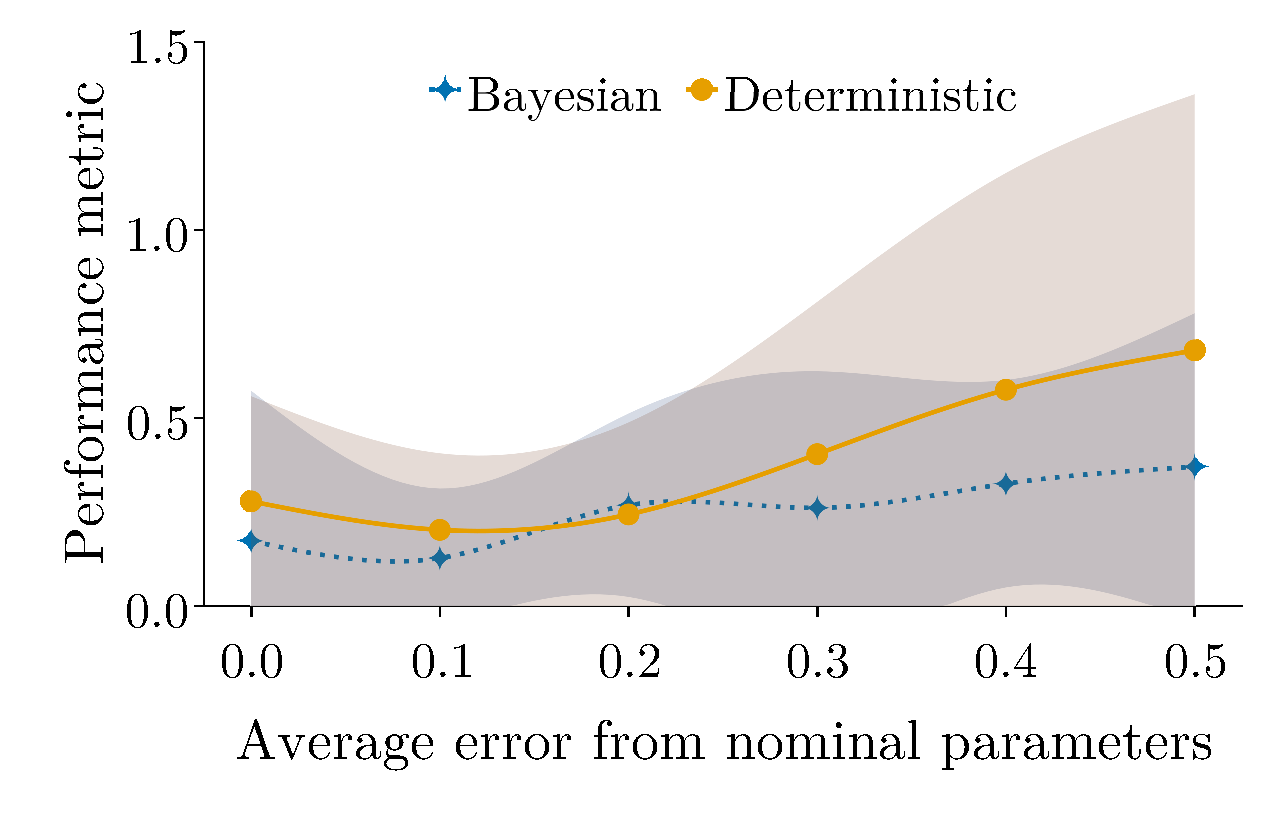
\includegraphics[clip,width=0.8\columnwidth]{./figures/bandplot2.eps}%
    \caption{\textsc{NeuralPbc} Performance metric ($J_T$) for various
    error in system parameters. Measurement noise included as Wiener process
    with standard deviation of $0.001$ and $0.02$ on joint angles and
    velocities, respectively}
    \label{fig:comparison_neuralpbc}
\end{figure}


\subsubsection{Real-World Experiments}

The controllers from both training schemes are evaluated on hardware. 
%
Since the nominal model~\eqref{eq:iwp_dynamics} neglects the friction in the
bearings any contribution to the dynamics by the belt-drive system, the hardware
experiments empirically demonstrate the robustness of our controllers against
these uncertainties.
%
We further bolster this claim by deliberately modifying the hardware and test
the controllers without any additional training.
%
In particular, throughout the experiments, the inertia wheel attached to $q_2$
is replaced with parts (labelled A-C on Table~\ref{tab:modified_params}) whose
mass and inertia are different from the nominal values.
%
The modified system parameters are summarized in
Table~\ref{tab:modified_params}.
%
% The parameter error listed on the last column of Table~\ref{tab:modified_params}
% is computed by $\|p - p_{\textrm{nom}}\| / \|p_{\textrm{nom}}\|$.
\begin{table}[tb]
  \centering
  \caption{System parameters used in real-world experiments. The errors in the
  last column are $\|p_s - p^{\textrm{nom}}_{s}\| / \|p^{\textrm{nom}}_{s}\|$}.
  % \rowcolors{2}{}{Wheat1}
  \begin{tabular}{lcccc}
    \toprule
    Parameter set $p_s$ & $I_1$ & $I_2$ & $mgl$ & Error \\
    \midrule
    Nominal & 0.0455 & 0.00425 & 1.795 & 0 \\
    A & 0.0417 & 0.00330 & 1.577 & $0.122$ \\
    B & 0.0378 & 0.00235 & 1.358 & $0.243$ \\
    C & 0.0340 & 0.00141 & 1.140 & $0.365$ \\
    \bottomrule
  \end{tabular}
  \label{tab:modified_params}
\end{table}
 
The system starts from rest at the downward position. 
%
A small disturbance in the $q_1$ direction is introduced to start the swing-up.
%
The state $x$ is recorded and~\eqref{eq:performance_metric} is the performance
metric used to evaluate the controllers.
%
% \begin{equation}
%     J_{\textrm{exp}}(x,u) = \frac{1}{2} \int_{0}^{T} 2 \bigl(1 - \cos q_1\bigr) + \dot{q}_1^2  + \dot{q}_2^2 + u^2 \, \dd t,
%     \label{eq:experiment_performance_metric}
% \end{equation}
%
% where $T$ is the time at which the switch to LQR occurs.
%
The results are summarized in Fig.~\ref{fig:neuralpbc_bar_plot}.


In all scenarios, our controllers are able to achieve the control objective
despite the errors introduced in the system parameters.
%
% Furthermore, the controller from Bayesian training consistently outperforms the
% controller from deterministic training, supporting the theoretical justification
% discussed in Section~\ref{ssec:justification}. 
%
These results demonstrate that our approach enables a unified way to tackle
nonlinear control problems while simultaneously incorporating prior knowledge
and model uncertainties.
%
\begin{figure}[t]
    \centering
    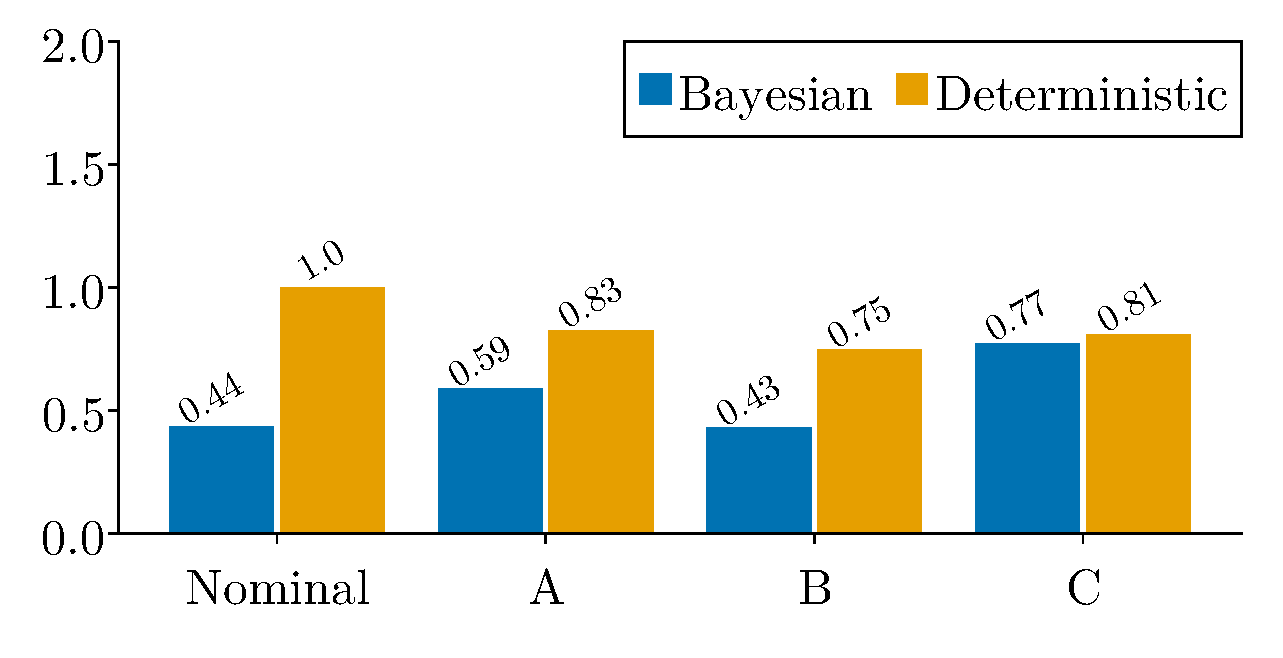
\includegraphics[width=0.9\linewidth]{pbc_bar.eps}
    \caption{
        %
        Controller performance for modified system parameters. 
        %
        The performance metric is given by
        Eq.~\eqref{eq:performance_metric}.
        %
        Lower values are better. 
        %
        These results show that controllers trained via Bayesian learning are
        consistently more robust to errors in system parameters.
        %
    }
    \label{fig:neuralpbc_bar_plot}
\end{figure}


% \begin{table}[t]
%     \centering
%     \caption{Comparison of the approaches}
%     \rowcolors{4}{}{Wheat1}
%     \begin{tabular}{lcc}
%       \toprule
%       & \multicolumn{2}{c}{Methods implemented} \\
%       \cmidrule(lr){2-3}
%       Case & Deterministic & Bayesian \\
%       \midrule
%       Robustness & \textcolor{red!88!green}{\xmark} & \textcolor{green!63!blue}{\cmark} \\
%       Computation cost & \textcolor{green!63!blue}{\cmark} &  \textcolor{red!88!green}{\xmark} \\
%       Model selection &  \textcolor{red!88!green}{\xmark} & \textcolor{green!63!blue}{\cmark} \\
%       Amount of data &  \textcolor{red!88!green}{\xmark} & \textcolor{green!63!blue}{\cmark} \\
%       Prior knowledge & \textcolor{green!63!blue}{\cmark} & \textcolor{green!63!blue}{\cmark}\textcolor{green!63!blue}{\cmark} \\
%       Learning stability & \textcolor{green!63!blue}{\cmark} &  \textcolor{red!88!green}{\xmark} \\
%       Overfitting &  \textcolor{red!88!green}{\xmark} & \textcolor{green!63!blue}{\cmark} \\
%       \bottomrule
%     \end{tabular}
%     \label{tab:comparison}
%   \end{table}

% \begin{minipage}{\textwidth}
%     \begin{minipage}[b]{0.45\textwidth}
%       \centering
%       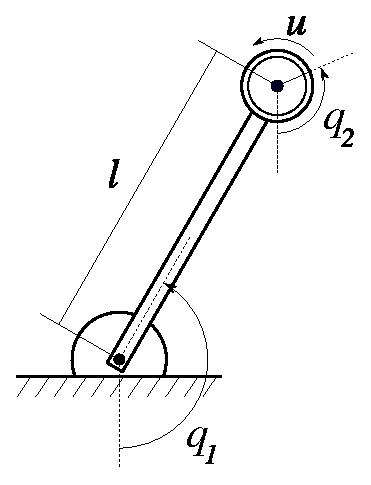
\includegraphics[width=0.5\textwidth]{figures/iwp.eps}
%       \captionof{figure}{Schematic of the inertia wheel pendulum. Only the rotating wheel \(\theta_2\) is actuated.}
%       \label{fig:iwp}
%     \end{minipage}
%     \hfill
%     \begin{minipage}[b]{0.45\textwidth}
%       \centering
%       \begin{tabular}{cc}\hline
%         Table head & Table head \\ \hline
%           Some values & Some values \\
%           Some values & Some values \\
%           Some values & Some values \\
%           Some values & Some values \\
%           Some values & Some values \\
%           Some values & Some values \\ \hline
%         \end{tabular}
%         \captionof{table}{A table beside a figure}
%         \label{tab:iwp_params}
%     \end{minipage}
% \end{minipage}

\subsection{Discussion}
\label{ssec:discussion}

Given a fixed amount of data available during a training session, the
deterministic framework has the upper hand since the Bayesian framework needs to
learn a whole probability distribution as opposed to a point summary of this
whole distribution. However, given a trustworthy prior distribution, Bayesian
framework needs much fewer data to come up with solutions that perform well. The
Bayesian framework is inherently more robust against parameter uncertainties and
measurement errors as long as the controller is computed by marginalizing the
probability distribution over the weights of the neural network as this process
is less prone to overfitting. Moreover, the Bayesian framework allows for
further training of the controller by updating the neural net parameters online;
that is, during the operation of the real system by treating the probability
distributions learned during simulation as priors.